\chapter{Методы передачи дискретных данных на физическом уровне}

При передаче дискретных данных по каналам связи применяются два основных типа физического кодирования - на основе синусоидального несущего сигнала и на основе последовательности прямоугольных импульсов.
Первый способ часто называется также \emph{модуляцией или аналоговой модуляцией}, а второй - \emph{цифровым кодированием}.

В настоящее время все чаще данные, изначально имеющие аналоговую форму - речь, телевизионное изображение, - передаются по каналам связи в дискретном виде, то есть в виде последовательности единиц и нулей.
Процесс представления аналоговой информации в дискретной форме называется дискретной модуляцией.
Термины <<модуляция>> и <<кодирование>> часто используют как синонимы.

\section{Аналоговая модуляция}

Аналоговая модуляция применяется для передачи дискретных данных по аналоговым каналам, типичным представителем которых является канал тональной частоты телефонных сетей.

% TODO: Uncomment after image adding
\begin{comment}
    Типичная амплитудно-частотная характеристика канала тональной частоты представлена на рисунке.

    Этот канал передает частоты в диапазоне от 300 до 3400 Гц, а его полоса пропускания составляет 3100 Гц, что обеспечивает приемлемое качество распознаваемости речи.
    Строгое ограничение полосы пропускания тонального канала связано с использованием частотной аппаратуры уплотнения.
\end{comment}

Устройство, которое выполняет модуляцию несущей на передающей стороне и демодуляцию на приемной, носит название модем (модулятор-демодулятор).

\subsection{Методы аналоговой модуляции}

\emph{Аналоговая модуляция} является таким способом физического кодирования, при котором информация кодируется изменением амплитуды, частоты или фазы синусоидального сигнала несущей частоты.

Основные способы аналоговой модуляции показаны на рисунке \ref{fig:types-of-analog-modulation}.
На диаграмме (а) показана последовательность бит исходной информации, представленная потенциалами высокого уровня для логической единицы и потенциалом нулевого уровня для логического нуля (потенциальным кодом).

\begin{figure}[!ht]
    \centering
    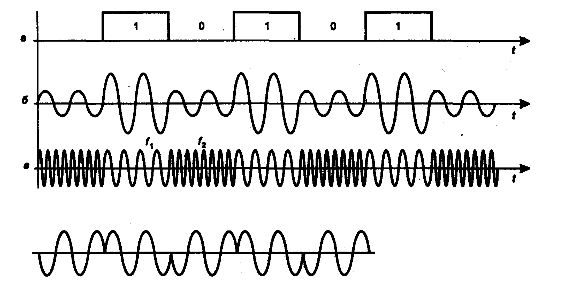
\includegraphics[width=0.8\textwidth]{types-of-analog-modulation}
    \caption{Различные типы аналоговой модуляции}
    \label{fig:types-of-analog-modulation}
\end{figure}

При \emph{амплитудной модуляции} (б) для логической единицы выбирается один уровень амплитуды синусоиды несущей частоты, а для логического нуля - другой.
Этот способ редко используется в чистом виде на практике из-за низкой помехоустойчивости, но часто применяется в сочетании с другим видом модуляции - фазовой модуляцией.

При \emph{частотной модуляции} (в) значения 0 и 1 исходных данных передаются синусоидами с различной частотой – $f_1$ и $f_2$.
Этот способ модуляции не требует сложных схем в модемах и обычно применяется в низкоскоростных модемах, работающих на скоростях 300 или 1200 бит/с.

При \emph{фазовой модуляции} (г) значениям данных 0 и 1 соответствуют сигналы одинаковой частоты, но с различной начальной фазой, например 0 и 180 градусов или 0, 90, 180 и 270 градусов.

В скоростных модемах часто используются комбинированные методы модуляции, как правило, амплитудная в сочетании с фазовой.

\subsection{Спектр модулированного сигнала}

Спектр результирующего модулированного сигнала определяется спектром модулирующей функции, который в свою очередь зависит от типа модуляции и скорости модуляции, то есть желаемой скорости передачи бит исходной информации.

При амплитудной модуляции спектр состоит из гармонической составляющей на несущей частоте $f_\text{с}$ и боковых составляющих $(f_\text{с} + n f_0)$ и $(f_\text{с} - n f_0)$, где $f_0$ - частота изменения информационного параметра синусоиды, $n = 1, 2, 3, 4, 5$ и т.д.
При использовании для модуляции прямоугольных импульсов и передаче последовательности чередующихся 1 и 0, амплитуды составляющих типа $(f_\text{с} + n f_0)$ и $(f_\text{с} - n f_0)$ убывают пропорционально $1 / n$, а $n$ - нечетное.
Обычно ограничиваются $n = 7$, а более высокими гармониками пренебрегают вследствие их малого вклада в результирующий сигнал.

При фазовой и частотной модуляции спектр сигнала получается более сложным, чем при амплитудной модуляции, но общий характер поведения спектральных составляющих сохраняется.

Для повышения скорости передачи данных используют комбинированные методы модуляции.
Наиболее распространенными являются методы квадратурной амплитудной модуляции (Quadrature Amplitude Modulation, QAM).
Эти методы основаны на сочетании фазовой модуляции с 8 значениями величин сдвига фазы и амплитудной модуляции с 4 уровнями амплитуды.
Однако из возможных 32 комбинаций сигнала используются далеко не все.
Такая избыточность кодирования используется для распознавания модемом ошибок, являющихся следствием искажений сигнала.

\section{Цифровое кодирование}

При \emph{цифровом кодировании} дискретной информации применяют \emph{потенциальные и импульсные коды}.

В \emph{потенциальных кодах} для представления логических единиц и нулей используется только значение потенциала сигнала, а его перепады, формирующие законченные импульсы, во внимание не принимаются.
\emph{Импульсные коды} позволяют представить двоичные данные либо импульсами определенной полярности, либо частью импульса - перепадом потенциала определенного направления.

\subsection{Требования к методам цифрового кодирования}

Методы цифрового кодирования должны удовлетворять одновременно следующим требованиям:
\begin{itemize}
    \item иметь минимальную ширину спектра результирующего сигнала при отсутствии постоянной составляющей;
    \item обеспечивать синхронизацию между передатчиком и приемником;
    \item обладать способностью распознавать ошибки;
    \item обладать низкой стоимостью реализации.
\end{itemize}

\emph{Более узкий спектр} сигналов позволяет на одной и той же линии (с одной и той же полосой пропускания) добиваться более высокой скорости передачи данных.
Кроме того, часто к спектру сигнала предъявляется требование отсутствия постоянной составляющей, то есть наличия постоянного тока между передатчиком и приемником.

\emph{Синхронизация передатчика и приемника} нужна для того, чтобы приемник точно знал, в какой момент времени необходимо считывать новую информацию с линии связи.
Эта проблема в сетях решается сложнее, чем при обмене данными между близко расположенными устройствами.
На небольших расстояниях хорошо работает схема, основанная на отдельной тактирующей линии связи.

\begin{figure}[!ht]
    \centering
    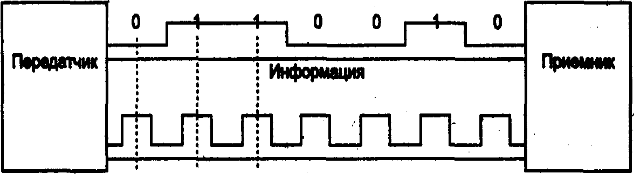
\includegraphics[width=0.8\textwidth]{little-distance-transiver-receiver-sync}
    \caption{Синхронизация приемника и передатчика на небольших расстояниях}
    \label{fig:little-distance-transiver-receiver-sync}
\end{figure}

В сетях использование этой схемы вызывает трудности из-за разброса времени прохождения сигнала вызванной неоднородностью характеристик проводников в кабелях.
Другой причиной, по которой в сетях отказываются от использования тактирующих импульсов, является экономия проводников в дорогостоящих кабелях.

Поэтому в сетях применяются так называемые \emph{самосинхронизирующиеся коды}, сигналы которых несут для передатчика указания о том, в какой момент времени нужно осуществлять распознавание очередного бита (или нескольких бит, если код имеет более чем два состояния информационного параметра сигнала).
Любой резкий перепад сигнала - так называемый фронт - может служить хорошим указанием для синхронизации приемника с передатчиком.

\emph{Распознавание и коррекцию искаженных данных} сложно осуществить средствами физического уровня, поэтому чаще всего эту работу берут на себя протоколы, лежащие выше: канальный, сетевой, транспортный или прикладной.
С другой стороны, распознавание ошибок на физическом уровне экономит время, так как приемник не ждет полного помещения кадра в буфер, а отбраковывает его сразу при распознавании ошибочных бит внутри кадра.

Требования, предъявляемые к методам кодирования, являются взаимно противоречивыми, поэтому каждый из рассматриваемых ниже популярных методов цифрового кодирования обладает своими преимуществами и своими недостатками по сравнению с другими.

\begin{figure}[!ht]
    \centering
    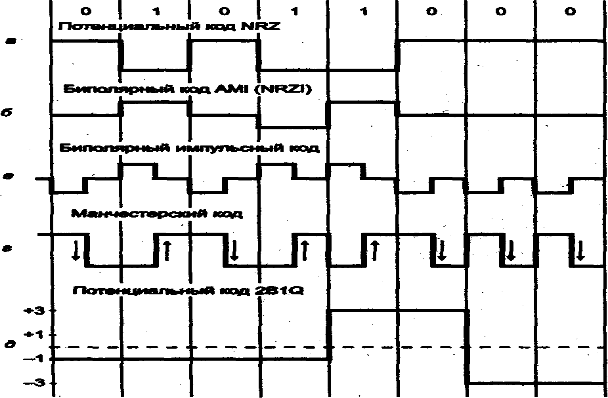
\includegraphics[width=0.7\textwidth]{discrete-code-signal}
    \caption{Вид сигнала в линии при использовании различных способов дискретного кодирования данных}
    \label{fig:discrete-code-signal}
\end{figure}

\subsection{Потенциальный код без возврата  к нулю}

Способ \emph{потенциального кодирования без возврата к нулю (Non Return to Zero, NRZ)} показан на эпюре (а).
Последнее название он получил потому, что при передаче последовательности единиц сигнал не возвращается к нулю в течение такта (как мы увидим ниже, в других методах кодирования возврат к нулю в этом случае происходит).

Способ NRZ прост в реализации, обладает хорошей распознаваемостью ошибок (из-за двух резко отличающихся потенциалов), имеет достаточно низкую частоту основной гармоники $f_0$, которая равна $N/2~Гц$, но не обладает свойством самосинхронизации.
При передаче длинной последовательности единиц или нулей потенциал на линии не изменяется, поэтому у приемника нет возможности определять по входному сигналу моменты времени, когда нужно в очередной раз считывать данные.

Другим серьезным недостатком является наличие низкочастотной составляющей, которая приближается к нулю при передаче длинных последовательностей единиц или нулей.
Из-за этого многие каналы связи, не обеспечивающие прямого гальванического соединения между приемником и источником, этот вид кодирования не поддерживают.

В результате в чистом виде код NRZ в сетях не используется, а применяются его различные модификации, в которых устраняют как плохую самосинхронизацию кода NRZ, так и наличие постоянной составляющей.

\subsection{Метод биполярного кодирования с альтернативной инверсией}

Одной из модификаций метода NRZ является \emph{метод биполярного кодирования с альтернативной инверсией (Bipolar Alternate Mark Inversion, AMI)}.
В этом методе (б) используются три уровня потенциала - отрицательный, нулевой и положительный.
Для кодирования логического нуля используется нулевой потенциал, а логическая единица кодируется либо положительным потенциалом, либо отрицательным, при этом потенциал каждой новой единицы противоположен потенциалу предыдущей.

Код AMI при передаче длинных последовательностей единиц ликвидирует проблемы наличия постоянной составляющей и отсутствия самосинхронизации, присущие коду NRZ, так как в этом случае сигнал на линии представляет собой последовательность разнополярных импульсов.
Длинные же последовательности нулей также опасны для кода AMI - сигнал вырождается в постоянный потенциал нулевой амплитуды.

В целом, для различных комбинаций бит на линии использование кода AMI приводит к более узкому спектру сигнала, чем для кода NRZ, а значит, и к более высокой пропускной способности линии
Код AMI предоставляет также некоторые дополнительные по сравнению с кодом NRZ возможности по распознаванию ошибочных сигналов.
Так, нарушение строгого чередования полярности сигналов говорит о ложном импульсе или исчезновении с линии корректного импульса.
Сигнал с некорректной полярностью называется запрещенным сигналом (signal violation).

В коде AMI используются не два, а три уровня сигнала на линии.
Дополнительный уровень требует увеличение мощности передатчика примерно на 3 дБ для обеспечения той же достоверности приема бит на линии, что является общим недостатком кодов с несколькими состояниями сигнала по сравнению с кодами, которые различают только два состояния.

\subsection{Потенциальный код с инверсией при единице}

Существует код, похожий на AMI, но только с двумя уровнями сигнала.
При передаче нуля он передает потенциал, который был установлен в предыдущем такте (то есть не меняет его), а при передаче единицы потенциал инвертируется на противоположный.
Этот код называется \emph{потенциальным кодом с инверсией при единице (Non Return to Zero with ones Inserted, NRZI)}.
Этот код удобен в тех случаях, когда использование третьего уровня сигнала весьма нежелательно, например, в оптических кабелях, где устойчиво распознаются два состояния сигнала - свет и темнота.

\subsection{Биполярный импульсный код}

В импульсных кодах данные представлены полным импульсом или же его частью - фронтом.
Наиболее простым случаем такого подхода является \emph{биполярный импульсный код}, в котором единица представлена импульсом одной полярности, а ноль - другой (в).
Каждый импульс длится половину такта.
Такой код обладает отличными самосинхронизирующими свойствами, но постоянная составляющая может присутствовать, например, при передаче длинной последовательности единиц или нулей.
Кроме того, спектр у него шире, чем у потенциальных кодов.
Так, при передаче всех нулей или единиц частота основной гармоники кода будет равна $N~Гц$, что в два раза выше основной гармоники кода NRZ и в четыре раза выше основной гармоники кода AMI при передаче чередующихся единиц и нулей.
Из-за слишком широкого спектра биполярный импульсный код используется редко.

\subsection{Манчестерский код}

В локальных сетях до недавнего времени самым распространенным методом кодирования был так называемый \emph{манчестерский код} (г).
Он применяется в технологиях Ethernet и Token Ring.

При манчестерском кодировании каждый такт делится на две части, а информация кодируется перепадами потенциала, происходящими в середине каждого такта.
Единица кодируется перепадом от низкого уровня сигнала к  высокому, а ноль - обратным перепадом.
В начале каждого такта может происходить служебный перепад сигнала, если нужно представить несколько единиц или нулей подряд.

Так как сигнал изменяется, по крайней мере, один раз за такт передачи одного бита данных, то манчестерский код обладает хорошими самосинхронизирующими свойствами.
Ширина спектра манчестерского кода уже, чем у биполярного импульсного.
У него также нет постоянной составляющей, а основная гармоника в худшем случае (при передаче последовательности единиц или нулей) имеет частоту $N~Гц$, а в лучшем (при передаче чередующихся единиц и нулей) она равна $N / 2~Гц$, как и у кодов AMI или NRZ.
В среднем ширина полосы манчестерского кода в полтора раза уже, чем у биполярного импульсного кода, а основная гармоника колеблется вблизи значения $3N / 4$.
Манчестерский код имеет еще одно преимущество перед биполярным импульсным кодом.
В последнем для передачи данных используются три уровня сигнала, а в манчестерском - два.

\subsection{Потенциальный код 2В1Q}

\emph{Потенциальный код с четырьмя уровнями сигнала} для кодирования данных показан на (д).
Это код 2B1Q, название которого отражает его суть - каждые два бита (2В) передаются за один такт сигналом, имеющим четыре состояния (1Q).
Паре бит 00 соответствует потенциал $-2,5~В$, паре  бит 01  соответствует  потенциал $-0,833~В$, паре 11 - потенциал $+0,833~В$, а паре 10 - потенциал $+2,5~В$.

При этом способе кодирования требуются дополнительные меры по борьбе с длинными последовательностями одинаковых пар бит, так как при этом сигнал превращается в постоянную составляющую.
При случайном чередовании бит спектр сигнала в два раза уже, чем у кода NRZ, так как при той же битовой скорости длительность такта увеличивается в два раза.
Таким образом, с помощью кода 2B1Q можно по одной и той же линии передавать данные в два раза быстрее, чем с помощью кода AMI или NRZI.
Однако для его реализации мощность передатчика должна быть выше, чтобы четыре уровня четко различались приемником на фоне помех.

\section{Логическое кодирование}

\emph{Логическое кодирование} используется для улучшения потенциальных кодов типа AMI, NRZI или 2B1Q.
Для логического кодирования, которое должно заменять длинные последовательности бит, приводящие к постоянному потенциалу, вкраплениями единиц, характерны два метода - \emph{избыточные коды и скрэмблирование}.

Первый метод основан на \emph{добавлении в исходный код избыточных бит}, содержащих логические единицы.
В этом случае длинные последовательности нулей прерываются, код становится самосинхронизирующимся для любых передаваемых данных и исчезает постоянная составляющая.
Но этот метод снижает полезную пропускную способность линии, так как избыточные единицы пользовательской информации не несут.

\emph{Другой метод основан на предварительном «перемешивании» исходной информации} таким образом, чтобы вероятность появления единиц и нулей на линии становилась близкой.
Устройства, или блоки, выполняющие такую операцию, называются скрэмблерами (scramble - свалка, беспорядочная сборка).
При скрэмб-лировании используется известный алгоритм, поэтому приемник, получив двоичные данные, передает их на дескрэмблер, который восстанавливает исходную последовательность бит.
Избыточные биты при этом по линии не передаются.

Оба метода относятся к логическому, а не физическому кодированию, так как форму сигналов на линии они не определяют.

\subsection{Избыточные коды}

\emph{Избыточные коды} основаны на разбиении исходной последовательности бит на символы, которые затем заменяют на новые символы, имеющие большее количество бит, чем исходные.
Например, логический код 4В/5В, используемый в технологиях FDDI и Fast Ethernet, заменяет исходные символы длиной в 4 бита на символы длиной в 5 бит.
Так как результирующие символы содержат избыточные биты, то общее количество битовых комбинаций в них больше, чем в исходных.
Так, в коде 4В/5В результирующие символы могут содержать 32 битовых комбинации, в то время как исходные символы - только 16.
Поэтому в результирующем коде можно отобрать 16 таких комбинаций, которые не содержат большого количества нулей, а остальные считать \emph{запрещенными кодами (code violation)}.
Кроме устранения постоянной составляющей и придания коду свойства самосинхронизации, избыточные коды позволяют приемнику распознавать искаженные биты.
Если приемник принимает запрещенный код, значит, на линии произошло искажение сигнала.

Соответствие исходных и результирующих кодов 4В/5В представлено ниже.

\begin{table}[!ht]
    \begin{tabular}{|c|c|c|c|}
        \hline
        \textbf{Исходный код} & \textbf{Результирующий код} & \textbf{Исходный код} & \textbf{Результирующий код} \\ \hline
        0000                  & 11110                       & 1000                  & 10010                       \\ \hline
        0001                  & 01001                       & 1001                  & 10011                       \\ \hline
        0010                  & 10100                       & 1010                  & 10110                       \\ \hline
        0011                  & 10101                       & 1011                  & 10111                       \\ \hline
        0100                  & 01010                       & 1100                  & 11010                       \\ \hline
        0101                  & 01010                       & 1100                  & 11011                       \\ \hline
        0110                  & 01110                       & 1110                  & 11100                       \\ \hline
        0111                  & 01111                       & 1111                  & 11101                       \\ \hline
    \end{tabular}
\end{table}

Буква В в названии кода означает, что элементарный сигнал имеет 2 состояния - от английского binary - двоичный.
Имеются также коды и с тремя состояниями сигнала, например, в коде 8В/6Т для кодирования 8 бит исходной информации используется код из 6 сигналов, каждый из которых имеет три состояния.

Для обеспечения заданной пропускной способности линии передатчик, использующий избыточный код 4В/5В, должен работать с тактовой частотой, повышенной на 25~\%.
Тем не менее, спектр избыточного потенциального кода оказывается уже спектра манчестерского кода, что оправдывает дополнительный этап логического кодирования, а также работу приемника и передатчика на повышенной тактовой частоте.

\subsection{Скрэмблирование}

Перемешивание данных скрэмблером перед передачей их в линию является другим способом логического кодирования.

Методы скрэмблирования заключаются в побитном вычислении результирующего кода на основании бит исходного кода и полученных в предыдущих тактах бит результирующего кода.
Например, скрэмблер может реализовывать следующее соотношение:
\[
    B_i = A_i \oplus B_{i-3} \oplus B_{i-5},
\]
где $B_i$ - двоичная цифра результирующего кода, полученная на $i\text{-м}$ такте работы скрэмблера, $A_i$ - двоичная цифра исходного кода, поступающая на $i\text{-м}$ такте на вход скрэмблера, $B_{i-3}$ и $B_{i-5}$ - двоичные цифры результирующего кода, полученные на предыдущих тактах работы скрэмблера, соответственно на 3 и на 5 тактов ранее текущего такта,  - операция исключающего ИЛИ (сложение по модулю 2).

Например, для исходной последовательности 110110000001 скрэмблер даст следующий результирующий код:

\begin{equation}
    \begin{aligned}
        & B_1    = A_1                          = 1 \\
        & B_2    = A_2                          = 1 \\
        & B_3    = A_3                          = 0 \\
        & B_4    = A_4    \oplus B_1            = 1 \oplus 1          = 0 \\
        & B_5    = A_5    \oplus B_2            = 1 \oplus 1          = 0 \\
        & B_6    = A_6    \oplus B_3 \oplus B_1 = 0 \oplus 0 \oplus 1 = 1 \\
        & B_7    = A_7    \oplus B_4 \oplus B_2 = 0 \oplus 0 \oplus 1 = 1 \\
        & B_8    = A_8    \oplus B_5 \oplus B_3 = 0 \oplus 0 \oplus 0 = 0 \\
        & B_9    = A_9    \oplus B_6 \oplus B_4 = 0 \oplus 1 \oplus 0 = 1 \\
        & B_{10} = A_{10} \oplus B_7 \oplus B_5 = 0 \oplus 1 \oplus 0 = 1 \\
        & B_{11} = A_{11} \oplus B_8 \oplus B_6 = 0 \oplus 0 \oplus 1 = 1 \\
        & B_{12} = A_{12} \oplus B_9 \oplus B_7 = 1 \oplus 1 \oplus 1 = 1 \\
    \end{aligned}
\end{equation}

Таким образом, на выходе скрэмблера появится последовательность 110001101111, в которой нет последовательности из шести нулей, присутствовавшей в исходном коде.
После получения результирующей последовательности приемник передает ее дескрэмблеру, который восстанавливает исходную последовательность на основании обратного соотношения, аналогичного исходному:
\[
    C_i = B_i \oplus B_{i-3} \oplus B_{i-5} = (A_i \oplus B_{i-3} \oplus B_{i-5}) \oplus B_{i-3} \oplus B_{i-5} = A_i.
\]

Существуют и более простые методы борьбы с последовательностями нулей и единиц, также относимые к классу скрэмблирования.

Для улучшения биполярного кода AMI используются два метода, основанные на \emph{искусственном искажении последовательности нулей запрещенными символами}.

\begin{figure}[!ht]
    \centering
    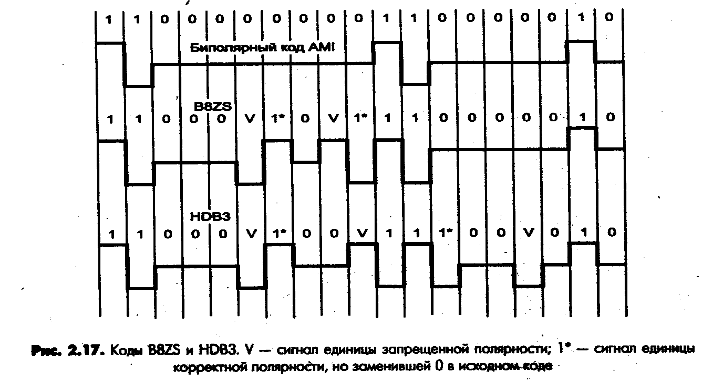
\includegraphics[width=0.8\textwidth]{B8ZS-and-HDB3-codes}
    \caption{Коды B8ZS и HDB3. V - сигнал единицы запрещённой полярности; $1^*$ "--- сигнал единицы корректной полярности, но заменившей 0 в исходном коде}
    \label{fig:B8ZS-and-HDB3-codes}
\end{figure}

Использовании метода B8ZS (Bipolar with 8-Zeros Substitution) и метода HDB3 (High-Density Bipolar 3-Zeros) для корректировки кода AMI иллюстрируется рисунком.
Исходный биполярный код AMI состоит из двух длинных последовательностей нулей, в первом случае - из 8, а во втором - из 5.

Код B8ZS (Bipolar with 8-Zeros Substitution) исправляет только последовательности, состоящие из 8 нулей.
Для этого он после первых трех нулей вместо оставшихся пяти нулей вставляет пять цифр: V1*0V1*.
V здесь обозначает сигнал единицы, запрещенной для данного такта полярности, то есть сигнал, не изменяющий полярность предыдущей единицы, 1* - сигнал единицы корректной полярности, а знак звездочки отмечает тот факт, что в исходном коде в этом такте была не единица, а ноль.
В результате на 8 тактах приемник наблюдает 2 искажения - очень маловероятно, что это случилось из-за шума на линии или других сбоев передачи.
Поэтому приемник считает такие нарушения кодировкой 8 последовательных нулей и после приема заменяет их на исходные 8 нулей.
Код B8ZS построен так, что его постоянная составляющая равна нулю при любых последовательностях двоичных цифр.

Код HDBЗ исправляет любые четыре подряд идущих нуля в исходной последовательности.
Правила формирования кода HDB3 более сложные, чем кода B8ZS.
Каждые четыре нуля заменяются четырьмя сигналами, в которых имеется один сигнал V.
Для подавления постоянной составляющей полярность сигнала V чередуется при последовательных заменах.
Кроме того, для замены используются два образца четырехтактовых кодов.
Если перед заменой исходный код содержал нечетное число единиц, то используется последовательность 000V, а если число единиц было четным - последовательность 1*00V.

Улучшенные потенциальные коды обладают достаточно узкой шириной спектра для любых последовательностей единиц и нулей, которые встречаются в передаваемых данных.
На рисунке приведены спектры сигналов разных кодов, полученные при передаче произвольных данных, в которых различные сочетания нулей и единиц в исходном коде равновероятны.
При построении графиков спектр усреднялся по всем возможным наборам исходных последовательностей.
Естественно, что результирующие коды могут иметь и другое распределение нулей и единиц.

Из рисунка видно, что потенциальный ход NRZ обладает хорошим спектром с одним недостатком - у него имеется постоянная составляющая.
Коды, полученные из потенциального путем логического кодирования, обладают более узким спектром, чем манчестерский, даже при повышенной тактовой частоте.
Заметим, что на рисунке спектр кода 4В/5В должен был бы примерно совпадать с кодом B8ZS, но он сдвинут в область более высоких частот, так как его тактовая частота повышена на 1/4 по сравнению с другими кодами.
Этим объясняется применение потенциальных избыточных и скрэмблированных кодов в современных технологиях, подобных FDDI, Fast Ethernet, Gigabit Ethernet, ISDN и т.п.
вместо манчестерского и биполярного импульсного кодирования.

\begin{figure}
    \centering
    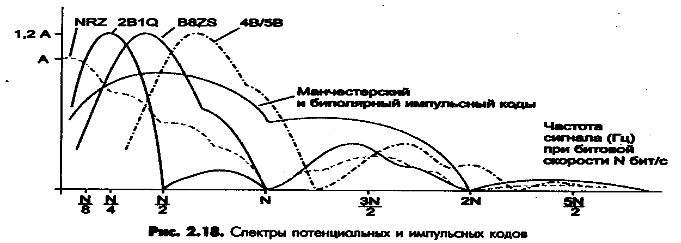
\includegraphics[width=0.9\textwidth]{potential-and-impulse-codes-spectres}
    \caption{Спектры потенциальных и импульсных кодов}
    \label{fig:potential-and-impulse-codes-spectres}
\end{figure}

\section{Дискретная модуляция аналоговых по источнику сигналов}

Одной из основных тенденций современного развития сетевых технологий является передача в сети как \emph{дискретных, так и аналоговых по источнику данных}.
На ранних этапах решения этой проблемы в территориальных сетях все типы данных передавались в аналоговой форме

Однако передача данных в аналоговой форме не позволяет улучшить качество принятых на другом конце линии данных, если они существенно исказились при передаче.
Преимуществом цифровых методов передачи информации является возможность контроля достоверности полученных по линии связи данных путем вычисления контрольной суммы, повторной передачи искаженных кадров, применения самокорректирующихся кодов.
Поэтому на смену аналоговой технике записи и передачи звука и изображения пришла цифровая техника, которая использует так называемую дискретную модуляцию исходных непрерывных во времени аналоговых процессов.

Дискретные способы модуляции основаны на дискретизации непрерывных процессов, как по амплитуде, так и по времени.
Рассмотрим принципы дискретной модуляции на примере \emph{импульсно-кодовой модуляции ИКМ (Pulse Amplitude Modulation, САМ)}, которая широко применяется в цифровой телефонии.

\subsection{Дискретная модуляция непрерывного процесса}

Текущие значения исходной непрерывной функции измеряются не непрерывно, а через фиксированные интервалы времени, которые называются \emph{периодами (интервалами) дискретизации}.
Этот процесс получил название дискретизации по времени.
Затем каждый замер, который получил название отсчета, представляется в виде двоичного числа определенной разрядности, при этом непрерывное множество возможных значений исходной аналоговой функции заменяется дискретным множеством ее значений.
Этот процесс получил название \emph{квантования по уровню}.
Устройство, которое выполняет подобную операцию, называется \emph{аналого-цифровым преобразователем (АЦП)}.
После этого отсчеты передаются по каналам связи двоичным кодом в виде последовательности единиц и нулей.

На приемной стороне линии с помощью \emph{цифро-аналогового преобразователя (ЦАП)} коды преобразуются в исходную непрерывную функцию времени.

Дискретная модуляции основана на \emph{теории отображения Найквиста - Котельникова}.
В соответствии с этой теорией, аналоговая непрерывная функция, переданная в виде последовательности ее дискретных по времени значений - отсчетов, может быть точно восстановлена, если частота дискретизации была в два или более раз выше, чем частота самой высокой гармоники спектра исходной функции.

В аналоговой телефонии для передачи голоса был выбран диапазон от 300 до 3400 Гц, который достаточно качественно передает все основные гармоники собеседников.
В соответствии с \emph{теоремой Найквиста - Котельникова} для качественной передачи голоса достаточно выбрать частоту дискретизации, в два раза превышающую самую высокую гармонику непрерывного сигнала, то есть 2 х 3400 - 6800 Гц.
Выбранная частота дискретизации 8000 Гц обеспечивает некоторый запас качества.

Для представления значения отсчета в методе ИКМ обычно используется 7 или 8 разрядов двоичного кода, что дает 128 или 256 градаций звукового сигнала.
При использовании метода ИКМ для передачи одного голосового канала необходима пропускная способность 56 или 64 Кбит/с, в зависимости от того, каким количеством бит (7 или 8) представляется каждый отсчет.

Стандартным является цифровой канал 64 Кбит/с, который также называется \emph{элементарным каналом цифровых телефонных сетей}.

Передача непрерывного сигнала в дискретном виде требует от сетей жесткого соблюдения временного интервала в 125 мкс (соответствующего частоте дискретизации 8000 Гц) между соседними замерами, то есть требует синхронной передачи данных между узлами сети.
При несоблюдении синхронности прибывающих замеров исходный сигнал восстанавливается неверно, что приводит к искажению голоса, изображения или другой мультимедийной информации.
Так, искажение синхронизации в 10 мс может привести к эффекту «эха», а сдвиги между замерами в 200 мс приводят к потере распознаваемости произносимых слов.
В то же время потеря одного замера при соблюдении синхронности между остальными замерами практически не сказывается на воспроизводимом звуке.

На качество восстановленного непрерывного сигнала влияет также и погрешность квантования значений отсчетов при использование для их представления двоичных чисел ограниченной разрядности.
Искажения восстановленного непрерывного сигнала за счет использования чисел конечной разрядности принято называть шумом квантования.

Представленные в цифровой форме непрерывные данные легко можно передать через компьютерную сеть.
Для этого достаточно поместить несколько замеров в кадр какой-нибудь стандартной сетевой технологии, снабдить кадр правильным адресом назначения и отправить адресату.
Адресат должен извлечь из кадра замеры и подать их с частотой квантования (для голоса - с частотой 8000 Гц) на ЦАП.
По мере поступления следующих кадров с замерами голоса операция должна повториться.
Если кадры будут прибывать достаточно синхронно, то качество голоса может быть достаточно высоким.
Однако, как мы уже знаем, кадры в компьютерных сетях могут задерживаться как в конечных узлах (при ожидании доступа к разделяемой среде), так и в промежуточных коммуникационных устройствах - мостах, коммутаторах и маршрутизаторах, что может привести к снижению качества передачи голоса в цифровой форме через компьютерные сети.

\section{Асинхронная и синхронная передачи}

При обмене данными на \emph{физическом уровне} единицей информации является бит, поэтому средства физического уровня всегда поддерживают \emph{побитовую синхронизацию} между приемником и передатчиком.

\emph{Канальный уровень} оперирует кадрами данных и обеспечивает \emph{синхронизацию между приемником и передатчиком на уровне кадров}.
В обязанности приемника входит распознавание начала первого байта кадра, распознавание границ полей кадра и распознавание признака окончания кадра.

Обычно достаточно обеспечить синхронизацию на указанных двух уровнях - битовом и кадровом, - чтобы передатчик и приемник смогли обеспечить устойчивый обмен информацией.
Однако при плохом качестве линии связи (обычно это относится к телефонным коммутируемым каналам) для повышения надежности передачи данных вводят дополнительную синхронизацию на уровне байт.

Такой режим работы называется \emph{aсинхронным} или \emph{старт-стопным}.
Другой причиной использования такого режима работы является наличие устройств, которые генерируют байты данных в случайные моменты времени.
Так работает клавиатура дисплея или другого терминального устройства, с которого человек вводит данные для обработки их компьютером.

\begin{figure}[!ht]
    \centering
    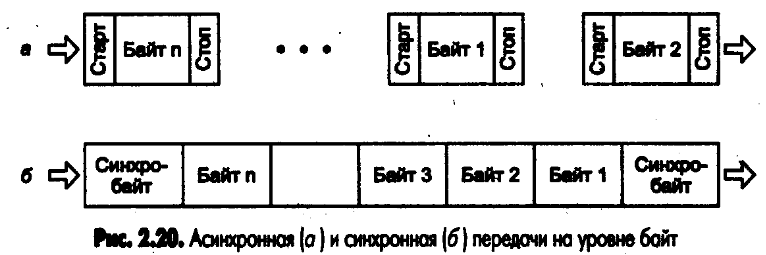
\includegraphics[width=0.9\textwidth]{async-and-sync-transmissions}
    \caption{Асинхронная (а) и синхронная (б) передачи на уровне байт}
    \label{fig:async-and-sync-transmissions}
\end{figure}

В асинхронном режиме каждый байт данных сопровождается специальными сигналами - «старт» и «стоп».
Назначение этих сигналов состоит в том, чтобы, во-первых, известить приемник о приходе данных и, во-вторых, чтобы дать приемнику достаточно времени для выполнения некоторых функций, связанных с синхронизацией, до поступления следующего байта.

Асинхронным описанный режим называется потому, что каждый байт может быть несколько смещен во времени относительно побитовых тактов предыдущего байта

При \emph{синхронном режиме} передачи старт-стопные биты между каждой парой байт отсутствуют.
Пользовательские данные собираются в кадр, который предваряется байтами синхронизации.
Байт синхронизации - это байт, содержащий заранее известный код, например 0111110, который оповещает приемник о приходе кадра данных.
При его получении приемник должен войти в байтовый синхронизм с передатчиком, то есть правильно понимать начало очередного байта кадра.
Так как при передаче длинного кадра у приемника могут появиться проблемы с синхронизацией бит, то в этом случае используются самосинхронизирующиеся коды.
